\section*{Chapitre 1 - Activité 1 : Retrouver les formules}

On rappelle que l'aire d'un rectangle se calcule avec la formule :

\prop{Rectangle}
    {\begin{figure}[H]
        \centering
        \begin{tikzpicture}
            \draw (0,0)--(3,0) node[midway,above] {$L$} ;
            \draw (0,0)--(0,-2) node[midway,left] {$l$} ;
            \draw (0,-2)--(3,-2) ;
            \draw (3,-2)--(3,0) ;
        \end{tikzpicture}
        $$l\times L$$
    \end{figure}}

\cnt Calculer les aires de chacune des figures suivantes.

    
\begin{minipage}[t]{0.25\textwidth}
    \begin{figure}[H]
        \centering
        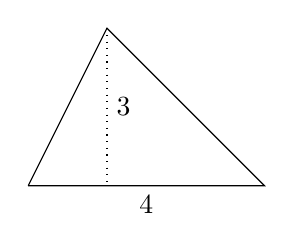
\begin{tikzpicture}
            \draw (0,0)--(1,2) --(3,0)--(0,0) node [midway, below] {$4$};
            \draw[dotted] (1,2)--(1,0) node [midway,right] {$3$};
            %\draw[dashed] (0,0) --(0,2)-- (3,2)--(3,0) ;
        \end{tikzpicture}
    \end{figure}
\end{minipage}
\hfill
\begin{minipage}[t]{0.25\textwidth}
    \begin{figure}[H]
        \centering
        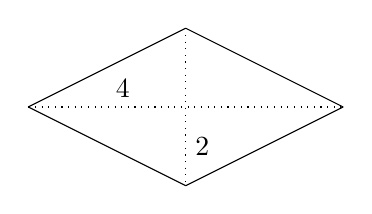
\begin{tikzpicture}
            \draw (0,0)--(2,1) node[midway,above,white] {$L$} ;%Pour alignement
            \draw (2,1)--(4,0);
            \draw [dotted] (0,0)--(4,0) ;
            \node at (1.2,0) [above] {$4$};
            \node at (2,-0.5) [right] {$2$};
            \draw [dotted] (2,1)--(2,-1) ;
            \draw (2,-1)--(4,0) ;
            \draw (2,-1)--(0,0) ;
        \end{tikzpicture}
    \end{figure}
\end{minipage}
\hfill
\begin{minipage}[t]{0.20\textwidth}
    \begin{figure}[H]
        \centering
        \begin{tikzpicture}[scale=0.9]
            \draw (-1,0)--(2,0) node[midway,above] {$4$} ;
            \draw (-1,0)--(0,-2);
            \draw[dotted] (1,0)--(1,-2)node[midway,left] {$3$} ;
            \draw (0,-2)--(3,-2) ;
            \draw (3,-2)--(2,0) ;
        \end{tikzpicture}
    \end{figure}
\end{minipage}
\hfill
\begin{minipage}[t]{0.20\textwidth}
\begin{figure}[H]
    \centering
    \begin{tikzpicture}
        \draw (0,0)--(2,0) node[midway,above,white] {$L$} ;%Pour alignement
        \draw (0,0)--(0,-2)node[midway,left] {$4$} ;
        \draw (0,-2)--(2,-2) ;
        \draw (2,-2)--(2,0) ;
    \end{tikzpicture}
\end{figure}
\end{minipage}

\cnt Pour chacune de ces figures, retrouver la formule générale permettant de calculer l'aire.